\chapter{Evaluation}

SynVisio was made publicly available to use for free on the internet on September 2018. A stable version was deployed in the start of 2019 and ever since then, it has been used by several researchers across the world in exploring genomic conservation in a wide variety of organisms. To evaluate our system we conducted semi-structured interviews with 5 domain experts from the three research groups we were collaborating with and one of the experts was a bioinformatician who worked across all three research groups. The interviews were conducted either through phone or an in person meeting and lasted around 45-60 minutes. Researchers were first asked about the relevance of synteny visualizations in their field of research and then asked to give their opinion on the different features that SynVisio offered and how they helped in exploring synteny in their particular datasets. We summarize their feedback of the system through three case studies, one from each research collaborator group, presented in the sections below. To provide evidence on the effectiveness of our system \textit{in the wild} we explored user activity logs on the website for a period of 12 months through google analytics. Finally to demonstrate the open-ended design of SynVisio we provide examples of genome databases for silk worm and two other species, that were extended to show synteny visualizations using the open sourced code of SynVisio.

\section{Case Studies}

\subsection{Wheat\textit{(Triticum aestivum)}}
What is one of the most widely cultivated crops in the world and plays an important role in human nutrition. Being a common cereal wheat genomes are highly diverse and spread over a large geographical range. The genome is capable of tolerating mutations and extensive hybridization to a great level which is why it has been able to adapt to such a wide variety of environmental conditions\cite{wheatinfo,10wheat}. Wheat is also one of the \textit{neolithic founder crops} that were the first to be domesticated almost 10000 years ago.
Bread wheat(AABBDD) is a hexaploid genome and is the result of series of hybridization events between three ancestral genomes A Donor\textit{(Triticum urartu)}, B Donor\textit{(Aegilops speltoides)} and D Donor\textit{(Aegilops tauschii)} which makes it an interesting subject for synteny analysis. Our collaborators were part of a research team involved in sequencing a high quality version of the wheat genome. Since the wheat genome is extremely large and complex synteny analysis can help researchers in assessing the quality and contiguity of the genome assembly though alignments between the sub genomes (A,B and D).

Our collaborators relied on visualizations generated by SynVisio to present and summarize their sequence assembly results - \textit{``the images have been used in presentations, academic meetings such as the international wheat congress and also at the plant-animal genome conference.'' (R1)}. While they used Circos style plots for research publications earlier, they mentioned that the multi level representations in SynVisio were far more useful for genomes like wheat with many chromosomes in it - \textit{``This tool is better than a Circos plot, especially when comparing multiple genomes, circos can be limited because you are seeing too many chromosomes in one circle and so are losing information ... a stacked layout like yours is easier to see.'' (R4)}. One collaborator in particular also appreciated the system for its ability to handle large datasets like wheat - \textit{``this is really neat. this is also very useful...a single wheat chromosome is vast and wheat has 21 of those placing stress on an analysis pipeline in terms of computational complexity...it is also very repetitive...'' (R1)}.
Feedback provided by this research team was also used in adding support for hive plots which offer a very intuitive representation to compare multiple sub genomes in crops like wheat as shown in figure \ref{fig:ch_6_wheat}. We have provided supporting material describing the process needed to generate this hive plot using SynVisio for this particular dataset through step by step screenshots of the system in the appendix. Our collaborators in this team plan on publishing images generated using SynVisio and have already used it to create a portal for researchers to compare 12 different wheat cultivars for the 10+ Wheat Genomes Project. Users can use this portal to select any two varieties from 12 different wheat cultivars and then compare genomic conservation between them using SynVisio\cite{10wheat,wheatinfogithub}.

\begin{figure}
  \centering
  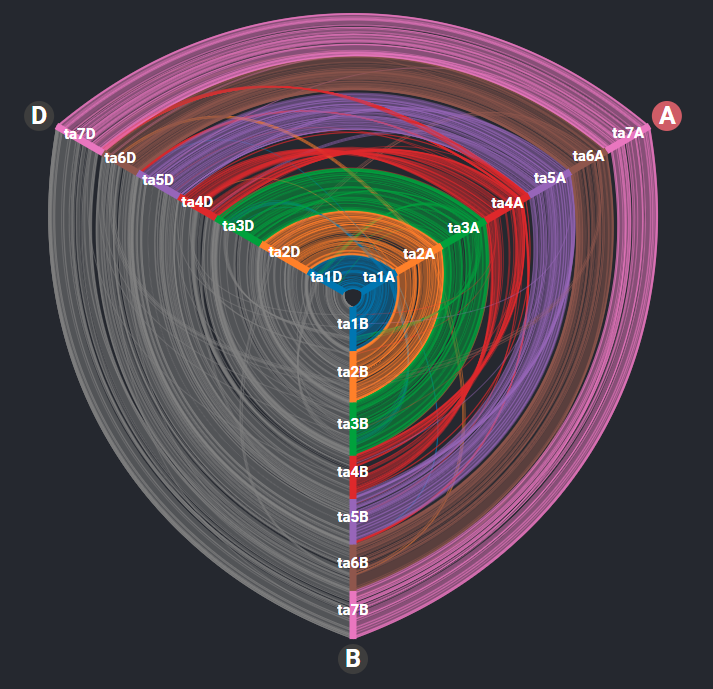
\includegraphics[width=0.65\linewidth]{images/ch_6_wheat.PNG}
  \captionof{figure}{Genomic conservation between the three sub genomes A,B and D of Wheat(Chinese Spring Variety) shown through a Hive plot in SynVisio.}
  \label{fig:ch_6_wheat}
\end{figure}


\begin{figure}
  \centering
  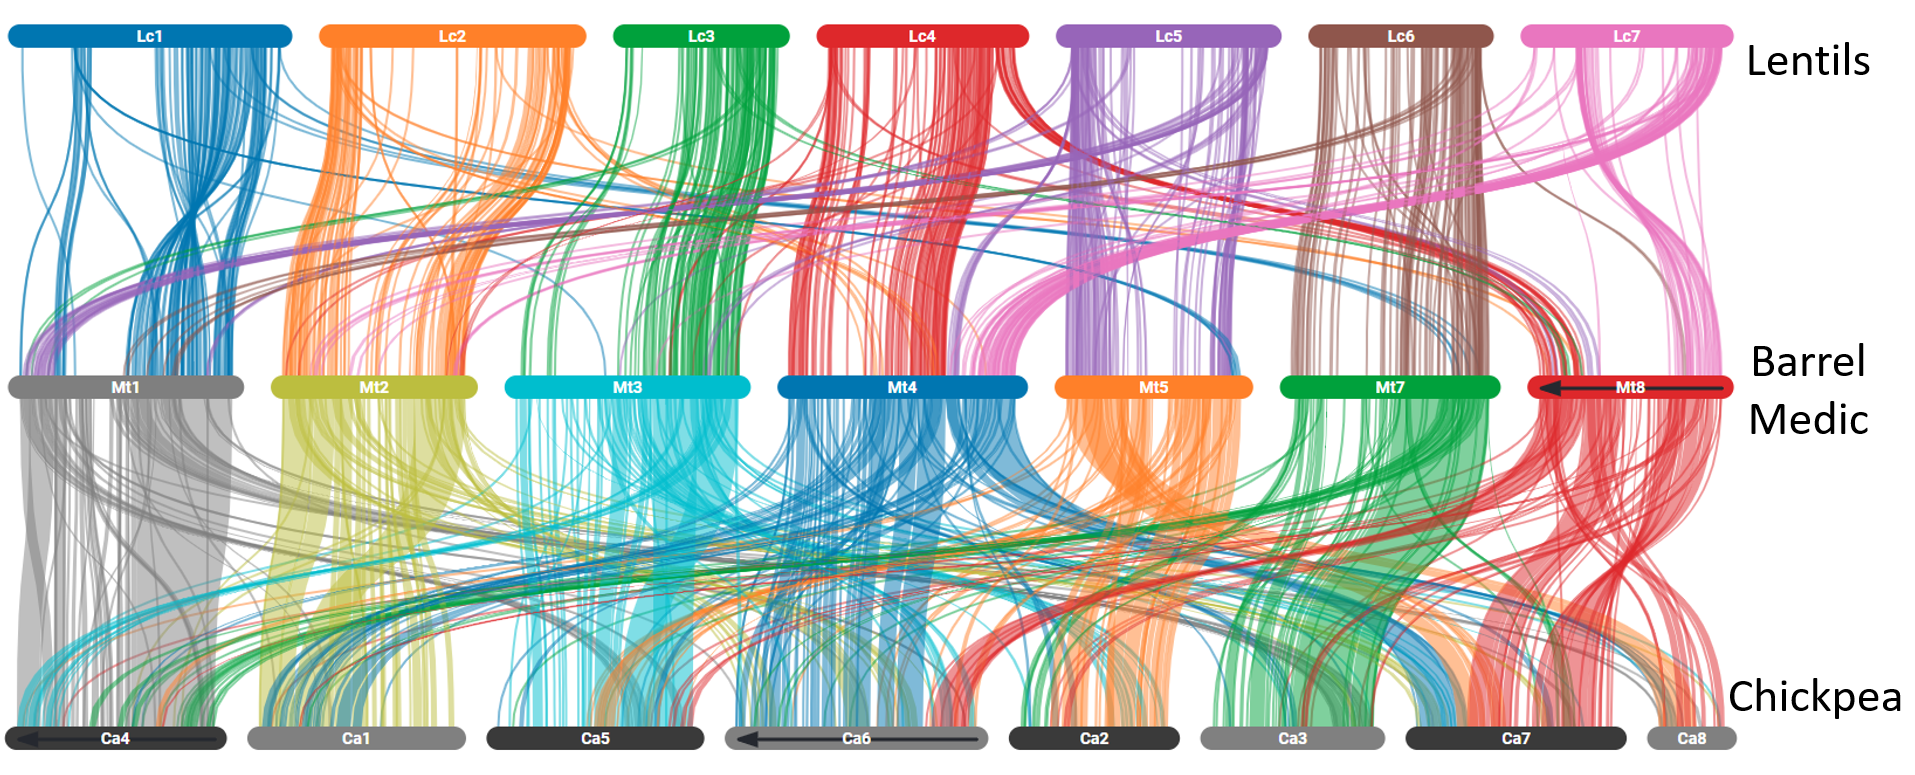
\includegraphics[width=1\linewidth]{images/ch_6_lentils.png}
  \captionof{figure}{Collinearity between Lentils(Lc), Barrel Medic(Mt) and Chickpea(Ca) presented through a Tree view plot. The ordering(Ca) and orientation(Mt8,Ca4 and Ca6 - flipped) of some chromosomes have been changed to reduce visual clutter.}
  \label{fig:ch_6_lentils}
\end{figure}


\subsection{Lentils\textit{(Lens culinaris)}}
Lentil is an important legume crop that is grown globally as a valuable source for dietary protein. It also plays a crucial role in food security in developing countries along with other legume crops like Chickpea\textit{(Cicer arietinum)}\cite{varshney2013draft}. Lentils can be made more resistant to diseases and weed infestations by increasing the genetic diversity of the genome through hybridization between disease resistant wild varieties. This however requires mapping the traits through molecular markers to assess their diversity. Our collaborators relied on comparative genomic mapping to leverage information from a model legume species like Barrel Medic(Medicago truncatula) onto less studied crop species like lentils and chickpea due to lack of common markers.

Unlike the wheat genome, synteny analysis requirements for this project were centered around cross synteny between species rather than self synteny. Due to the large size difference in the genomes between Lentils(4Gbp) and Chickpea(~740Mbp) the first version of SynVisio was not able to generate legible charts as the Lentil chromosomes were extremely wide compared to chromosomes from the other species and so a special feature was added to have variable scales at different levels. Our collaborators were pleased with the updated view and also remarked on the multiple visual representations provided in the genome view - \textit{``I think it's quite good, I do really like that there's also the dot plot, in the corner, so that if anything is a little bit unclear, from the parallel view, you can kind of refer back to that.
'' (R5)}. Because this was a cross synteny analysis between several genomes, researchers mentioned that the Tree view was particularly helpful in summarising large scale chromosomal rearrangements and inversions while still keeping the different genomes visually distinct as shown in figure \ref{fig:ch_6_lentils}. They also compared it to circos plots and remarked on its usability - \textit{``It's like the circos plots are beautiful but you can't do anything with it. Whereas this, the tree-view in particular, is very aesthetically pleasing and that's the kind of thing that you can show to your collaborators and you can also understand it, at the same time, and then the interactive nature of it helps too...
(R5)''}. Reseachers froom this group have also used SynVisio to study genomic conservation in other legumes like the Tepary Bean\textit{(Phaseolus acutifolius)} and are planing on using it to generate images for their research publications in future.

\subsection{Canola\textit{(Brassica napus)}}
Canola is an important oil seed crop in the world as it is an excellent source for both animal feed and high quality edible oil\cite{shahidi1990canola}.It is an allotetraploid (4 copies - AACC) species that was formed through interspecific hybridization between diploid ancestors Brassica rapa (A Donor) and Brassica oleracea (C Donor)\cite{parkin1995identification}. Studying this genomic conservation can help researchers in looking at genetic variations that are advantageous from an evolutionary perspective in polyploids like Canola. Our collaborators from this research group were particularly interested in using comparative mapping to understand the level of genome duplication in modern brassica cultivars and the occurrence of genomic rearrangement in the evolution of these varieties from a common ancestor. This meant that they needed to visualize both self synteny between Canola itself and also cross synteny between canola and its closely related species. - \textit{``...in polyploid plants where there are many genomic rearrangements, visualization is really useful because there is lots of information and its really complicated for us to understand without an overview... (R2)''.}

SynVisio also helped researchers in this team at refining their assemblies - \textit{``Our assembly got better when we upgraded our sequencing from short read to long read sequencing technology as more regions are assembled. This tools helps us visualize that improvement ...(R2)''}. Regarding the visual representations one collaborator remarked that the parallel plot representation was better at showing genomic conservation than dot plots - \textit{``We have always used dot plots but these (parallel plots) are visually more intuitive...when chromosomes start breaking apart its much more difficult to follow where things are going in that big square and in this its easier to play around...Its much easier to trace things and work out where you are...(R3)''}. Researchers from this team have used visualizations generated by SynVisio at several conferences such as PAG (Plant Animal Genome) 2019 \cite{brassicapag} and also in a recent publication describing long read assemblies of two diploid Brassica species\cite{perumal2020high}.
 
\section{Global Usage Analysis}

Although our system was initially designed based on requirements from our collaborators for use within our university it was made publicly available as an open access tool on the internet and has been used since then by researchers across the world in a wide variety of research projects and images generated by SynVisio have also been used in research publications describing new genome assemblies and annotations\cite{mathers2020improved,perumal2020high}.

To quantify the use of SynVisio since it was made public we analysed web traffic through google analytics  from Jan 1st 2019 to Jan 1st 2020. In this period of 12 months SynVisio had 154 unique users spanning 267 sessions with an average session duration for each session being around 2 minutes while some users spent as much as 28 minutes on the system exploring different datasets. Users were from 18 different countries across the world as shown in Figure \ref{fig:ch_6_users} with a majority of the users being from China(53) followed by the United States(45) and Canada(23) respectively.

\begin{figure}
  \centering
  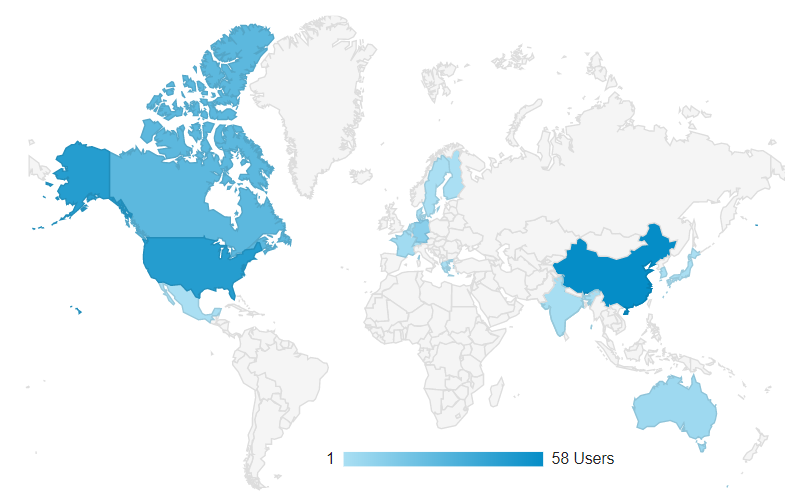
\includegraphics[width=1\linewidth]{images/ch_6_users.PNG}
  \captionof{figure}{Global user distribution of SynVisio for a period of 12 months from 2019-2020.}
  \label{fig:ch_6_users}
\end{figure}


SynVisio was designed in a modular fashion as a reusable component and its source code was open-sourced through an MIT license on GitHub\cite{synvisio}, which meant that it could be adopted and reused in other research tools and projects. An example of a system that has used SynVisio in this manner is \textbf{TeaBase} an online genome database with various tools, one of which is SynVisio, to explore the Tea plant(\textit{Camellia sinensis}) genome as shown in Figure \ref{fig:ch_6_other}\cite{teabase}. Other genome databases that have used SynVisio in a similar manner are \textbf{VitisGDB} and  \textbf{SilkDB 3.0} to explore the genomes of Grapevine and Silkworm respectively\cite{lu2020silkdb,vitisgdb}.

\begin{figure}[h]
  \centering
  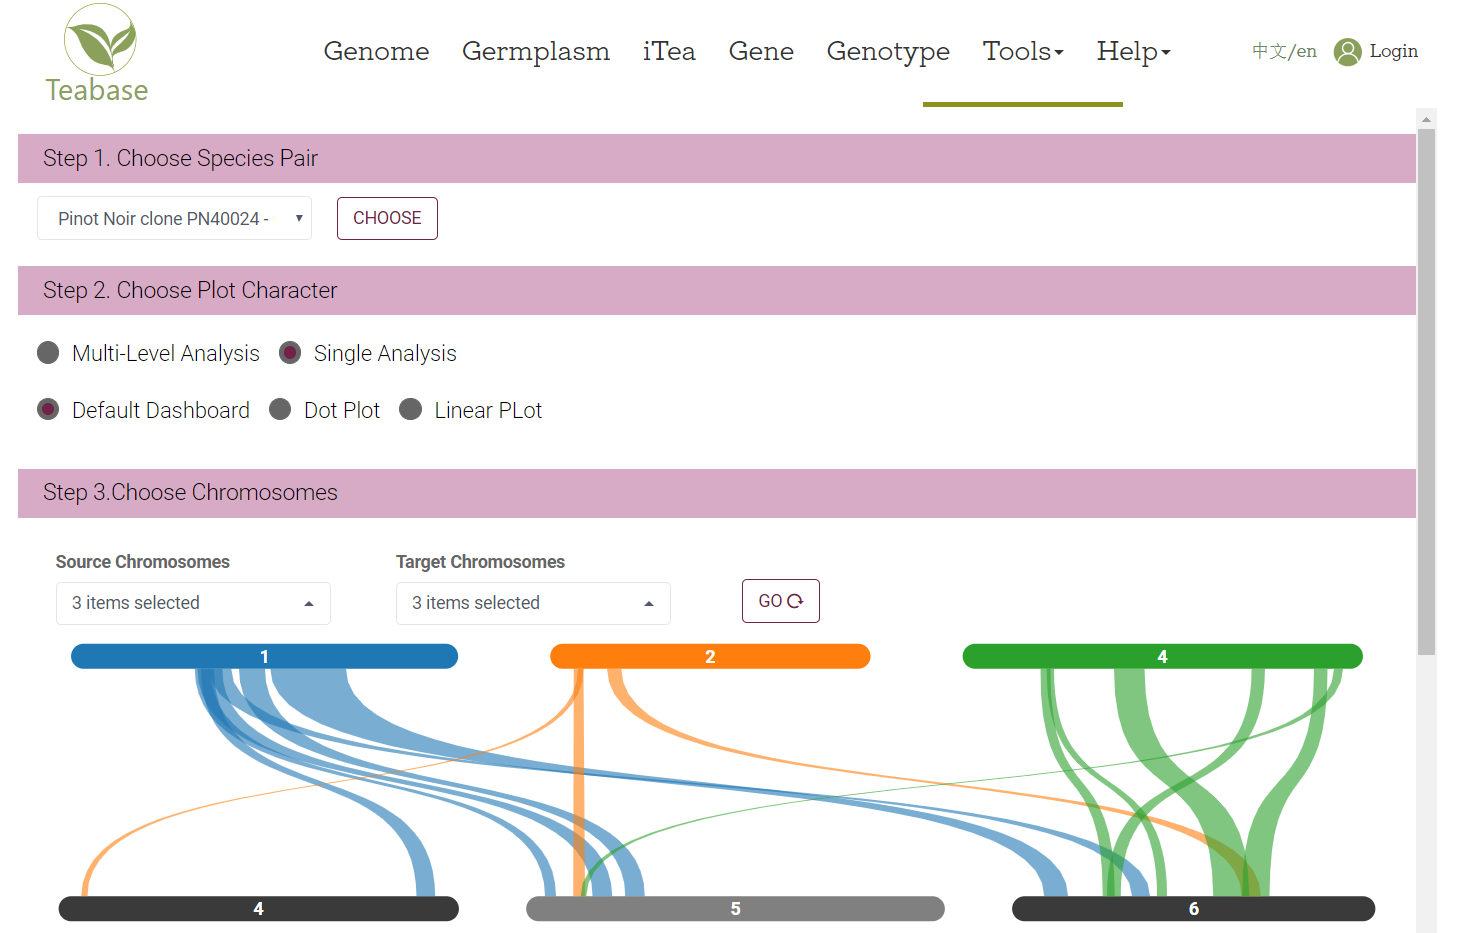
\includegraphics[width=1\linewidth]{images/ch_6_other.PNG}
  \captionof{figure}{TeaBase, an online genome database to explore the Tea plant genome with a modified version of SynVisio adapted into its toolset. }
  \label{fig:ch_6_other}
\end{figure}


\section{Evaluation Summary}  
Although several visualization tools exist for analysing genomic conservation they arent easily accessible as mentioned by researchers we interviewed -  \textit{``There are a couple of R based tools that we use but none of them are as complete as synvisio (R4)''}. SynVisio has been able to fill this critical gap
- \textit{``There isnt anything like this. Especially not where you can play around with your dataset. (R3)''}. When asked to rate SynVisio for its ability to visualize genomic conservation across different levels on a scale of 1(very bad) to 5(very good), 4 researchers gave the system the highest rating of 5 and one researcher gave it a rating of 4 stating that they would have liked greater control over the ordering and orientation of the chromosomes. This feedback validates the usability of the system for the initial set of visual tasks we designed the system for. Further we were also able to meet the supplementary design requirements that we had envisioned for data refinement and enhancement. Although some researchers mentioned that they did not find the filter panel quite helpful \textit{``I do most of my filtering ahead of time before running the tool so this filter is personally not useful for me but I can see why you have it...
 (R4)''} others found use for it - \textit{``The images are quite messy and it (filter panel) is definitely helpful in cleaning it up a bit... (R3)''}, \textit{``When looking for distant relatives, the feature with E value filter is useful.(R2)''}. 
 
Making SynVisio an online tool with the ability to directly upload sequences to visualize them has improved the usability of the tool to a great extent as several researchers mentioned that this has allowed them to share their work with other collaborators easily -\textit{`` if I wanted to discuss some of the results of this with a collaborator, I just zip up the two files that you need for input. Send it off to them and they can put it in and play with it themselves(R5)''}. This is also further evident by the web traffic SynVisio has received since its has been made available on the internet. Further the system design has also been adopted in several online genome databases, showing that it is a valuable tool in exploring genomes and interacting with them.



